This element is used for tracking through an arbitrary magnetic field
when its values are known at regularly spaced grid points and it is
hard to find a suitable model to describe it. The input magnet
parameter and coordinate system definition are illustrated in
Fig:\ref{fig:ftable_mag}. 

The \verb|THRESHOLD| parameter sets the magnitude of magnetic field below which the
field is considered zero. If this is too small, there may be numerical problems.

The field data is provided in an SDDS file, with two formats available. The recommended
format can be used if the \verb|SIMPLE_INPUT| parameter is non-zero.

\paragraph{Simple input format} --- This format is shared with the \verb|BMXYZ| element
and is more convenient than the original, default format.
The field map file is an SDDS file with the following columns:
\begin{itemize}
\item {\bf x}, {\bf y}, {\bf x} --- Transverse coordinates in meters (units should be ``m'').
\item {\bf Bx}, {\bf By}, {\bf Bz} --- Field values in Tesla (units should be ``T'').
\end{itemize}

The field map file must contain a rectangular grid of points,
equispaced (separately) in x, y, and z.  There should be no missing values
in the grid (this is not checked by {\tt elegant}).  In addition, the
x values must vary fastest as the values are accessed in row order, then the y values.
To ensure that this is the case, use the following command on the field
file:
\begin{flushleft}
sddssort {\em fieldFile} -column=z,incr -column=y,incr -column=x,incr
\end{flushleft}

N.B.: Particles are injected into the field region with z=0. Hence, one would normally want
the minimum value of z to be 0.

\paragraph{Original input format} --- This format is difficult to understand and
set up. Although it is not recommended, it is the default at present for historical
reasons.

The field data is saved in a 3 pages ($B_x$,
$B_y$, $B_z$) 3D histogram SDDS table (see \verb|MHISTOGRAM| for detail).
An example is shown in Fig:\ref{fig:ftable_input}.
This SDDS file must have one column \verb|Frequency| to store the
field data in Tesla, and following parameters:

\begin{itemize} 
\item \verb|ND| --- Type ``long''; Value ``3''.
\item \verb|Variable00Name|, \verb|Variable01Name|,\verb|Variable02Name| 
      --- Type ``string''; Value ``x'', ``y'', ``z''.
\item \verb|Variable00Min|, \verb|Variable01Min|, \verb|Variable02Min|
      --- Type ``double''; Value: the minimum boundary coordinates of
      ``x'', ``y'', ``z'' in meter. \verb|Variable02Min| (z\_min) must start from zero.
\item \verb|Variable00Max|,\verb|Variable01Max|, \verb|Variable02Max| 
      --- Type ``double''; Value: the maximum boundary coordinates of 
      ``x'', ``y'', ``z'' in meter.
\item \verb|Variable00Interval|, \verb|Variable01Interval|,\verb|Variable02Interval|
      --- Type ``double''; Value of the grid size of ``x'', ``y'', ``z'' in meter.  
\item \verb|Variable00Dimension|,\verb|Variable01Dimension|, \verb|Variable02Dimension|
      --- Type ``long''; Value of total number of grid points in
      ``x'', ``y'', ``z''.  For example: Variable00Dimension
      =(Variable00Max-Variable00Min)/Variable00Interval + 1.
\end{itemize}

N.B.: Particles are injected into the field region with z=0. Hence, one would normally want
\verb|Variable02Min|=0. If \verb|Variable02Min|$<$0, data ahead of the injection point.

\begin{figure}[htbp] 
  \begin{center}
  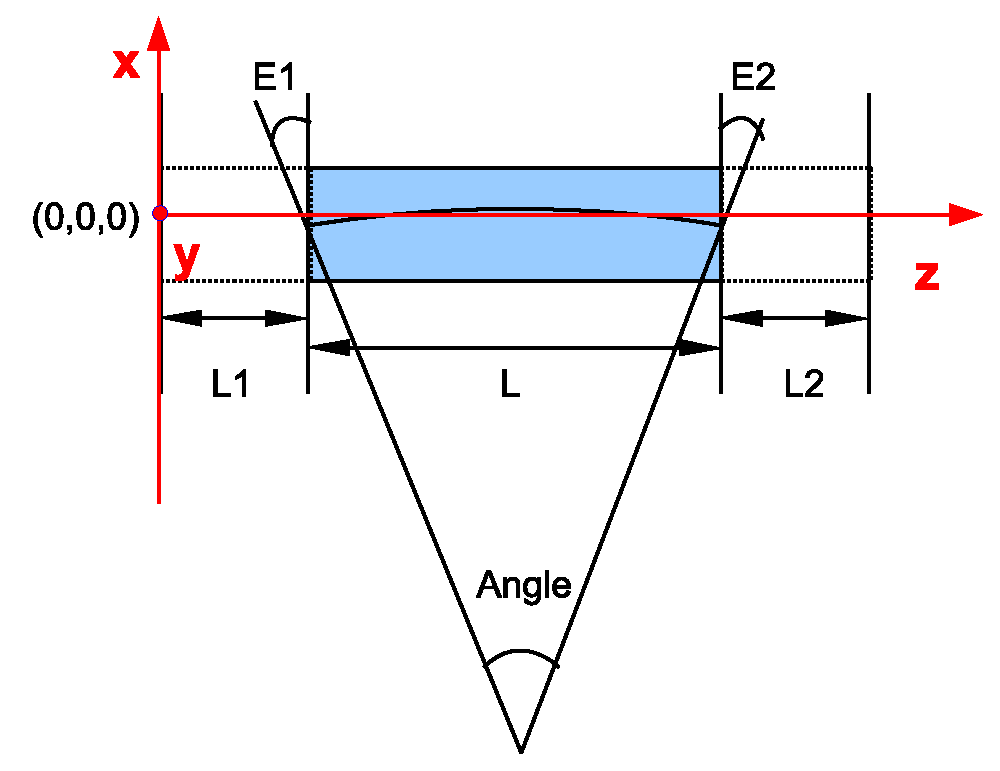
\includegraphics[width=3in,height=2.5in]{ftable-fig1.eps}
  \caption{\label{fig:ftable_mag} Illustration of coordinate
      system and magnet definition.}  
   \end{center} 
\end{figure}

\begin{figure}[htbp] 
  \begin{center}
  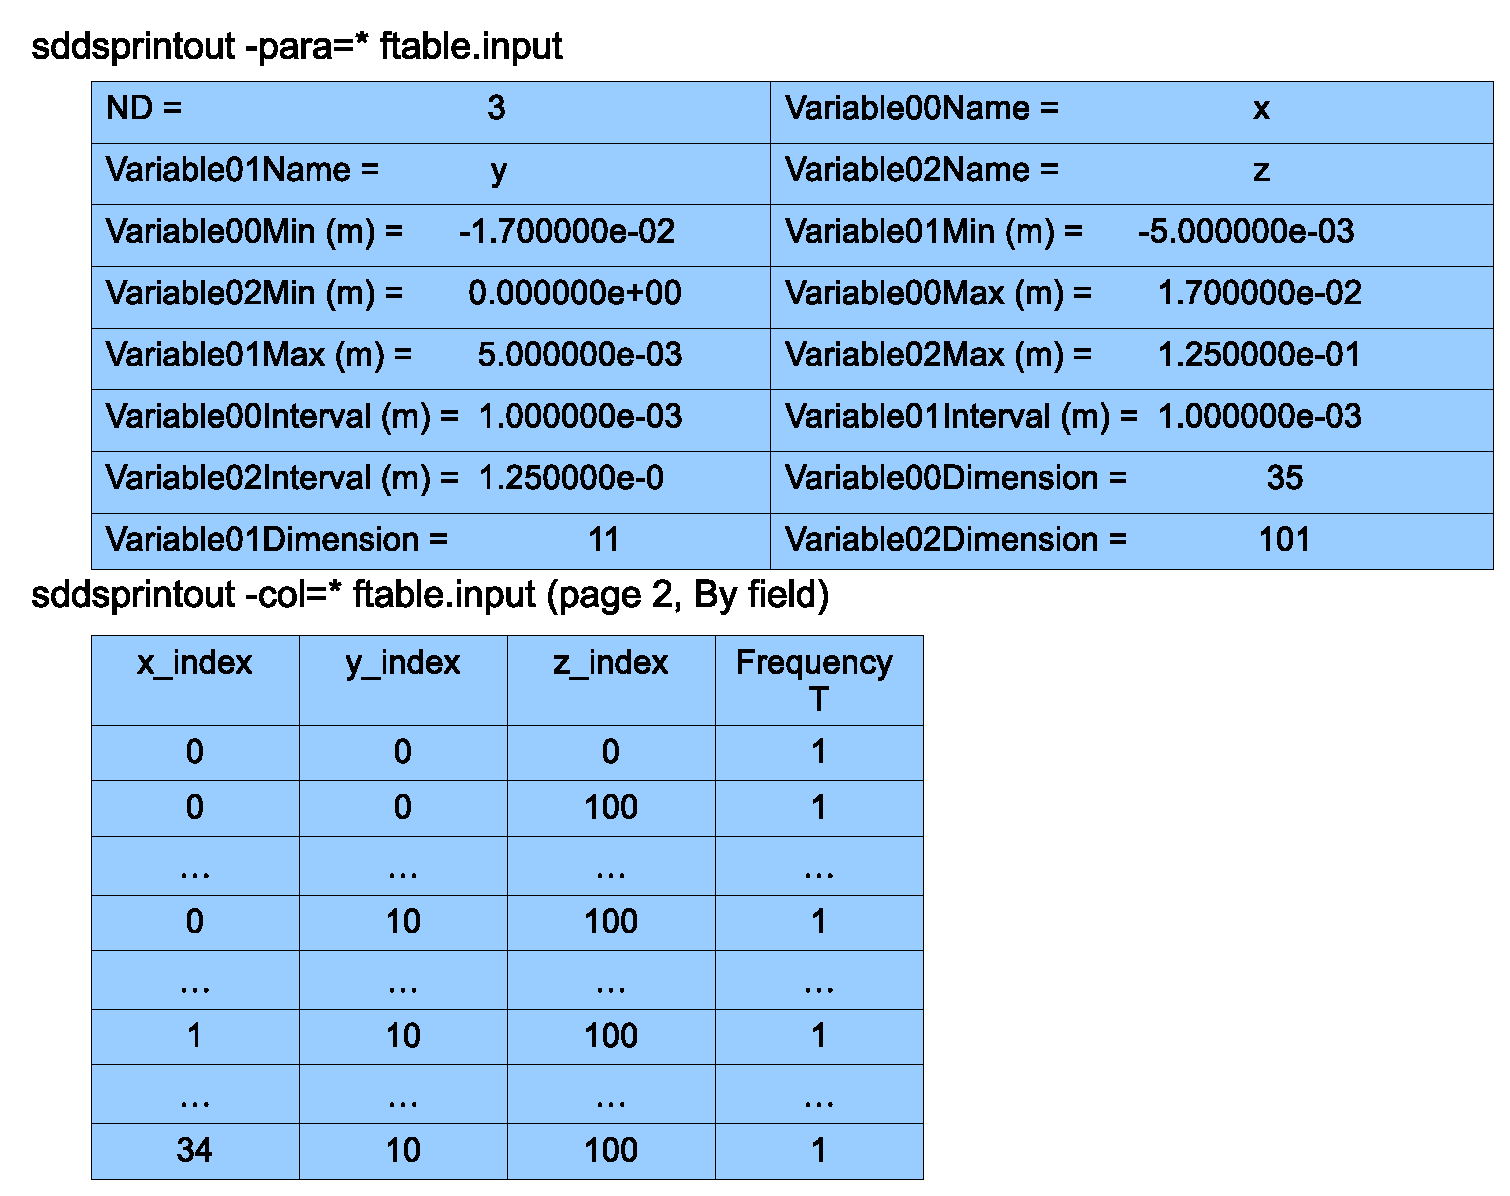
\includegraphics[width=6.5in,height=5.5in]{ftable-fig2.eps}
  \caption{\label{fig:ftable_input} Example of SDDS input
      file. The column x\_index, y\_index, z\_index is not the necessary
      part, it's shown here just for clarifying how the data is
      arranged} 
  \end{center} 

\end{figure}
